%%
%% Capítulo 2: Regras gerais de estilo
%%

\mychapter{Fundamentação científico-tecnológica}
\label{Cap:fundamentacao}

\section{Contextualização e problema}
\label{contextualização}

% Falar um pouco sobre o cenário mundial de eólica

% Falar sobre o problema com desempenho das máquinas

% Falar das tecnologias utilizadas

% Falar da robustez do sistema

% Falar do valor agregado

O setor energético é o principal insumo dos mais variados setores da economia, sendo item fundamental para o desenvolvimento econômico e social. Para que este setor consiga acompanhar e alavancar os avanços da sociedade, devemos investir cada vez mais em desenvolvimento de novas tecnologias, bem como aumentar o acesso da sociedade às fontes mais eficientes e limpas de energia.

A energia eólica é vista como uma das mais promissoras fontes de energia, pela sua crescente utilização e investimentos, tendo apresentado nos últimos anos uma evolução exponencial da capacidade eólica instalada. Atualmente os países lideres em geração de energia eólica são, China, Estados Unidos da América e Alemanha. Em 2010 a China tornou-se o país com a maior capacidade instalada no mundo, sendo atualmente responsável por 35\% do total da capacidade instalada, seguida pelos Estados Unidos, que possuem 17\% do total \cite{global-wind-energy}. Na figura \ref{Fig:ranking-mundial-capacidade-instalada} é demonstrado o ranking mundia de capacidade instalada, no qual o Brasil ocupa a 8ª posição.

\begin{figure}[htbp!] \begin{center}
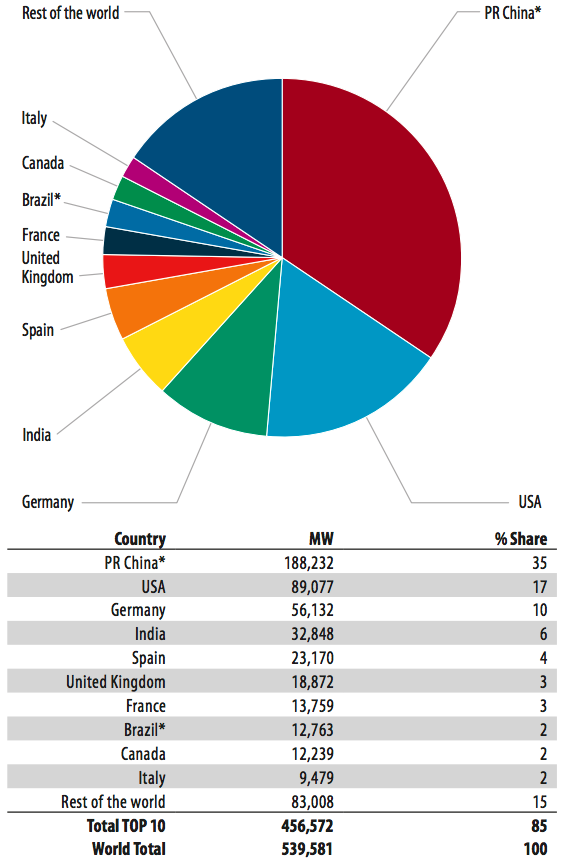
\includegraphics[width=0.75\linewidth]{./figuras/grafico-capacidade-instalada-mundo}
\caption{Ranking mundia de capacidade instalada}
\label{Fig:ranking-mundial-capacidade-instalada}
\end{center} 
\end{figure}

O Brasil recebe destaque no cenário mundial pelo elevado potencial eólico e pelo volume de geração de energia por fonte eólica, que tem crescido consideravelmente nos últimos anos. Com 508 usinas no total, o ano de 2017 terminou com 12,77 GW de potência eólica instalada, o que representou um crescimento de 18,87\% de potência em relação a dezembro de 2016, quando a capacidade instalada era de 10,74 GW \cite{boletim-anual-geracao-2017}.

Em 2017 foram instalados no país 6,84 GW de potência, considerando todas as fontes de geração de energia elétrica. Desse crescimento, 47,86\% corresponde a fonte hidroelétrica e 29,62\% a fonte eólica. Com esse acréscimo de 2,03 GW de capacidade instalada, o total eólico permitiu para a fonte uma participação de 8,10\% da matriz elétrica brasileira, como pode ser observado no gráfico \ref{Fig:matriz-energetica-brasileira}, que apresenta a participação de todas as fontes de geração na matriz elétrica brasileira no final de 2017 \cite{boletim-anual-geracao-2017}.

\begin{figure}[htbp!] \begin{center}
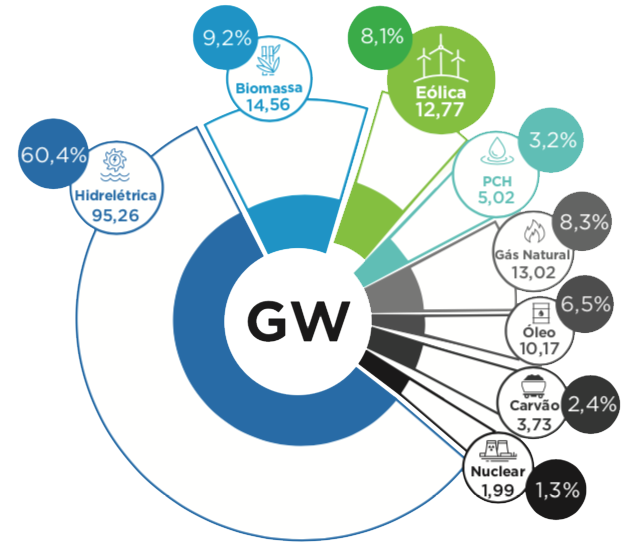
\includegraphics[width=0.65\linewidth]{./figuras/matriz-energetica-brasileira}
\caption{Matriz energética brasileira}
\label{Fig:matriz-energetica-brasileira}
\end{center} 
\end{figure}

Sendo um dos países que mais investe em energia eólica no mundo, o Brasil também é considerado um dos mais atrativos para investimentos em energias renováveis. A fonte eólica, sozinha, foi responsável por cerca de 80\% dos investimentos em renováveis no país de 2005 até 2015 \cite{CENARIO}. Um dos maiores motivos do alto investimento em energia eólica no Brasil é o alto valor do fator de capacidade proporcionado pelos ventos brasileiros. O fator de capacidade aponta o aproveitamento do vento para produção de energia e é representado pela proporção entre a geração efetiva da usina em um intervalo de tempo e a sua potência instalada. Em 2017 o valor médio do fator de capacidade no Brasil foi de 42,9\%, tendo atingido maior fator mensal médio em setembro, com 60,6\%, enquanto que no restante do mundo a média do é de 24,7\% \cite{boletim-anual-geracao-2017}.

O crescimento da utilização da força dos ventos para a produção de energia atribui-se principalmente ao desenvolvimento tecnológico no setor, que elevou a competitividade em relação ao preço, quando comparado com outras fontes geradoras de energia elétrica \cite{matrizes-energeticas-brasil}. Entretanto, a implantação de parques eólicos ainda exige um alto nível de investimento. Com o crescimento do mercado e da concorrência, o valor de remuneração obtido nesses empreendimentos tem sido cada vez menor, fazendo com que os investidores não possam tolerar qualquer problemas no desempenho dos aerogeradores e buscar ao máximo reduzir os riscos associados ao negócio.

Monitorar continuamente o funcionamento de um parque eólico permite ao gestor de um parque eólico uma visão mais ampla do que esta acontecendo na sua produção. O maior benefício que isso pode trazer é detectar desempenhos insatisfatórios, identificar e corrigir os problemas que causaram esses desvios e com isso, evitar perdas na receita. Além disso, o conhecimento e os ensinamentos adquiridos ao longo do monitoramento podem ser de grande utilidade no projeto, na construção e na operação de outros parques.

O contributo social desta pesquisa é fornecer uma ferramenta que irá possibilitar o monitoramento contínuo de parques eólicos, visando o aumento da eficiência desses parques, conferindo, consequentemente, maior competitividade para a fonte eólica frente às demais fontes de geração, o que pode estimular a modicidade tarifária, a qual preconiza o consumo de energia mais barata para o cidadão brasileiro. Além disso, incentivar a expansão de fontes renováveis de energia, que não agridem o meio ambiente, é contribuir para o bem-estar humano.

% Focar mais no problema

\subsection{Conceitos preliminares}
\label{Sec:conceitosPreliminares}

\subsubsection{O aerogerador}
\label{Sec:oAerogerador}

Aerogeradores basicamente são dispositivos projetados para transformar energia cinética dos ventos em algum tipo de energia mecânica. Os aerogeradores podem ser classificados de acordo com a orientação de seu rotor entre aerogerador de eixo vertical ou de eixo horizontal.

A maioria dos aerogeradores modernos utilizados comercialmente possuem em sua maioria eixo horizontal, três pás e um sistema de transmissão baseado em caixa multiplicadora. A figura \ref{Fig:ilustracaoAerogerador} ilustra os principais componentes de um aerogerador. São eles:

\begin{itemize}
    \item \textbf{Rotor:} Localizado no topo da torre, é composto pelo conjunto do hub e das pás. É o responsável por transferir a energia do vento através do torque para o eixo principal.
    \item \textbf{Nacele:} Compartimento instalado no alto da torre que armazena os elementos responsáveis pala conversão da energia mecânica em energia elétrica.
    \item \textbf{Torre:} Elemento que sustenta o rotor e a nacele na altura apropriada ao seu funcionamento.
    \item \textbf{Yaw:} Sistema responsável pela rotação da nacele (controle de giro), especialmente para o posicionamento do rotor de forma perpendicular à direção do vento.
    \item \textbf{Sistema de transmissão:} Composto pelo eixo principal e a caixa multiplicadora. O eixo principal transmite o torque gerado a partir da rotação das pás em uma frequência baixa. A caixa multiplicadora é responsável por elevar esta frequência de rotação até a entrada do gerador. Existem modelos de aerogeradores denominados de \textit{direct drive}, o torque do rotor é levado diretamente ao gerador, eliminando a necessidade de uso de caixa multiplicadora.
    \item \textbf{Sistema Elétrico:} Composto por toda a parte de conversão, transmissão de energia e controle do aerogerador. O principal subcomponente deste sistema é o gerador.
\end{itemize}

\begin{figure}[htbp!] \begin{center}
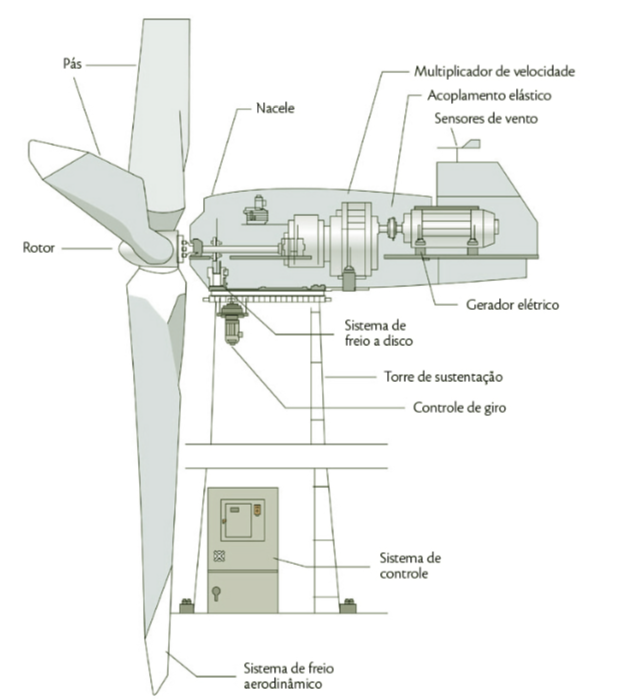
\includegraphics[width=0.75\linewidth]{./figuras/ilustracao-aerogerador}
\caption{Componentes de um aerogerador}
\label{Fig:ilustracaoAerogerador}
\legend{Fonte: \cite{componentes-aerogerador}}
\end{center} 
\end{figure}

\subsubsection{Sistema SCADA}
\label{Sec:scada}

Os Sistemas SCADA (Supervisory Control and Data Aquisition), ou sistemas supervisórios, são sistemas comumente utilizados na automação industrial que utilizam computação e comunicação para automatizar o monitoramento e controlar processos industriais. Eles permitem que os dados de um determinado processo produtivo sejam monitorados e rastreados. Esses dados são coletadas continuamente através de sensores e posteriormente, enviados para o computador central que faz o gerenciamento dos dados.

Os sistemas supervisórios são essenciais para o funcionamento de um parque eólico. Através deles os operadores conseguem controlar e armazenar os dados dos aerogeradores, torres anemométricas e subestações. Dentre os dados armazenados pelo sistema SCADA são encontrados informações da potência, da velocidade do vento na nacele, a orientação da nacele, temperaturas, pressões, entre outros. A partir desses dados contidos no SCADA é possível identificar falhas, calcular a quantidade de energia gerada, ter acesso a disponibilidade dos aerogeradores, etc.


\subsubsection{Curva e coeficiente de potência}
\label{Sec:curvaDePotencia}

A potência de uma turbina eólica varia de acordo com a velocidade do vento e cada turbina tem uma curva característica de desempenho de energia. Com essa curva é possível prever a produção de energia de um aerogerador, sem considerar detalhes técnicos de seus componentes. Assim, a curva de potência é um gráfico que indica qual a potência elétrica disponível no aerogerador para diferentes velocidades de vento \cite{iec-power-performance}.

Nas curvas de potência de um aerogerador estão definidas 3 zonas importantes:

\begin{itemize}
  \item \textit{Cut-in:} Representa a zona de arranque do aerogerador. Geralmente entre 2 e 4 m/s. Abaixo dessa velocidade não interessa extrair energia.
  \item \textit{Velocidade nominal:} Velocidade de vento que permite obter uma potência próxima da nominal. Normalmente entre 12 e 15 m/s
  \item \textit{Cut-out:} Velocidade de vento que o aerogerador é desligado por questões de segurança relacionadas a esforços mecânicos a que fica sujeito. Geralmente para velocidades de vento superiores a 25 m/s
\end{itemize}

A quantidade de potência disponível no vento que pode ser convertida em potência mecânica por um aerogerador, é chamado de coeficiente de potência ($c_p$). Esse coeficiente indica é utilizado para comparar a eficiência entre diferentes aerogeradores. Na figura \ref{Fig:ilustracaoCurvaPotencia} é demonstrado o gráfico com a curva e o coeficiente de potência de um aerogerador. 

\begin{figure}[htbp!] \begin{center}
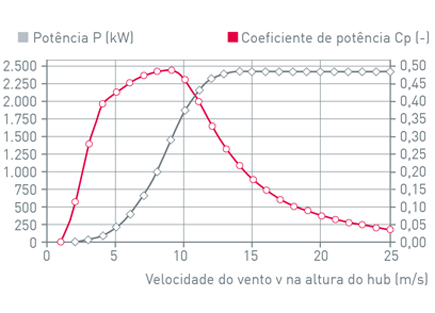
\includegraphics[width=0.75\linewidth]{./figuras/curva-potencia-wobben}
\caption{Curva de potência de um aerogerador}
\label{Fig:ilustracaoCurvaPotencia}
\legend{Fonte: \cite{catalogo-wobben-e92}}
\end{center} 
\end{figure}

\subsection{Desempenho de aerogeradores}
\label{Sec:desempenhoDeAerogeradores}

O risco de um investimento em um parque eólico esta fortemente atrelado as diferenças entre a produção efetiva e a produção estimada durante a elaboração do projeto. A partir disso surge a necessidade do acompanhamento do funcionamento dos parques eólicos para que seja garantido o bom desempenho dos aerogeradores.

A metodologia aplicada para o acompanhamento do desempenho dos parques, na maioria das vezes está prevista no contrato entre a empresa dona do parque eólico e a empresa fabricante dos aerogeradores e nesse caso essa verificação assume também um caráter de garantia no qual eventuais desvios podem originar penalizações, caso o desempenho seja abaixo do contratual.

A grande maioria dos contratos entre os fabricantes e os parques eólicos levam em consideração a disponibilidade dos aerogeradores como parâmetro para acompanhamento do desempenho. Esse indicador não é efetivo para medir o desempenho e sim apenas uma contabilização do tempo em que as máquinas estiveram em operação ou em condições de operação. É um conceito que não permite saber se foi produzido toda a energia que poderia ter sido produzida para as condições de vento verificadas.

Segundo \citeasnoun{metodologia-avaliacao-desempenho-de-parques}, a medição do desempenho só foi verdadeiramente introduzida em um parque eólico quando se passou a associar a disponibilidade com a medição da curva de potência dos aerogeradores, levando em consideração as condições de funcionamento que essas máquinas foram submetidas no seus locais de instalação. Com isso as diversas perdas existentes em um parque eólico (elétricas, aerodinâmicas, falhas, etc) passaram a ser contabilizadas e a detecção de situações que antes não eram analisadas passaram a ganhar mais notoriedade.

O desempenho de um aerogerador depende essencialmente da sua curva de potência e da sua disponibilidade. 

\subsubsection{Curva de potência}
\label{Sec:curvaPotenciaDesempenhoAerogeradores}

Como mencionado anteriormente, a curva de potência de um aerogerador é uma curva característica que expressa a potência gerada em função da velocidade do vento. Essa ferramenta é essencial para avaliação de desempenho de um aerogerador, tanto para previsão de produção, como para avaliação dos resultados obtidos. Entretanto, a curva de potência garantida pelo fabricante de aerogerador e a curva obtida com a turbina em funcionamento nem sempre são iguais. Além do local onde é feita a garantia da curva de potência e do local onde opera o aerogerador serem diferentes, existem outras razões pelas quais podem existir desvios no comportamento da curva de potência. Algumas razões são:

\begin{itemize}
  \item \textbf{Turbulência:} Pode ser definida como alterações na média da velocidade do vento em curtos períodos de tempo (ordem de segundos ou menos). Normalmente é gerada por conta da fricção com a superfície, causado pela topografia, e efeitos térmicos, por conta da variação da temperatura.
  \item \textbf{Efeito esteira:} Uma vez que a turbina eólica produz energia mecânica a partir da energia do vento incidente, o vento que "sai" da turbina tem um conteúdo energético muito menor que o do vento que "entrou". Pode ser definida como alterações na média da velocidade do vento que passou pelo rotor, podendo diminuir até um terço da velocidade inicial, formando uma esteira de vento turbulento. O diâmetro da esteira aumenta conforme o vento se afasta do rotor e se dissolve com uma distância média de 10 diâmetros do rotor.
  \item \textbf{Operação com limitação de potência:} Toda as turbinas são desenvolvidas com algum sistema de controle de potência. Para evitar danos ao equipamento é necessário limitar a potência mecânica do aerogerador durante ventos com velocidade acima da velocidade nominal de operação. Caso essa limitação de potência ocorrer por um longo período de tempo, trará prejuízos consideráveis ao parque eólico.
  \item \textbf{Deterioração e danificação nas pás:} A função das pás é converter, através da força de sustentação, a energia cinética do vento em energia mecânica. O seu desenho é feito para converter o máximo de energia possível, logo, o desgaste desta ao longo do tempo claramente afeta o desempenho aerodinâmico, afetando a sustentação gerada e consequentemente a potência retirada.
  \item \textbf{Condições climáticas:} Condições climáticas imprevistas podem afetar o desempenho de um aerogerador. Um exemplo são as baixas temperaturas, onde o gelo formado nas pás podem alterar o desempenho aerodinâmico, levando a perda energética. Outros casos que podem afetar o desempenho são a presença de insetos ou poeira, nas pás da turbina.
\end{itemize}

\subsubsection{Disponibilidade}
\label{Sec:disponibilidadeDesempenhoAerogeradores}

Pode-se dizer, de uma maneira geral, que a disponibilidade de um aerogerador esta relacionada com a avaliação da sua capacidade em desempenhar a função para o qual foi projetado, gerar energia. Devido a falhas de controle, problemas técnicos ou paradas para manutenção, os aerogeradores não estão todo tempo disponíveis para gerar energia. Com isso, durante a operação de um parque eólico, é necessário medir o quanto cada aerogerador ficou disponível para geração.

Esse conceito pode no entanto ser interpretado de formas diferentes. Por um lado existem os fabricantes dos aerogeradores, que estão interessados em avaliar o período em que as turbinas se apresentaram operacionais, desde que se verifiquem as condições externas de meteorologia e da rede elétrica, para os quais foram projetados. Do outro lado exite o proprietário do parque, que valoriza mais o tempo de operação perdido em vez das razões que levaram a essa perda. Estes dois pontos de vistas formam os dois principais conceitos de disponibilidade em energia eólica: disponibilidade técnica, na perspectiva do fabricante e disponibilidade operacional, na perspectiva do proprietário. Em resumo, a principal diferença entre as duas visões está relacionado a causa de cada parada dos aerogeradores e, consequentemente, no nível de garantia esperada pelos proprietários e que os fabricantes podem não estar dispostos a assegurar.

As diferenças entre a abordagem do fabricante e a do proprietário de um aerogerador geram discussões sobre os contratos de manutenção de um parque, que contemplam a definição da disponibilidade mínima a atingir (geralmente 97\% para a média da disponibilidade anual do conjunto de todos os aerogeradores de um parque), assim como as penalidades no caso de não comprimento.

A definição das metodologias usadas para estimar a energia não produzida em consequência da redução da disponibilidade é praticamento o tema mais sensível dos contratos entre o fabricante e o proprietário dos aerogeradores.

\citeasnoun{wind-turbine-availabily}, propõem um novo cálculo para a disponibilidade levando em consideração a energia produzida. Ao invés de calcular o tempo em que o aerogerador deixou de produzir, calcula-se a energia que deixou de ser produzida. As falhas de funcionamento nos aerogeradores tendem a ocorrer quando eles são mais solicitados, ou seja, quando a velocidade do vento é elevada, assim, \citeasnoun{wind-turbine-availabily} mostram que a disponibilidade com base na energia tende a ser superior à disponibilidade com base no tempo.

\subsection{Monitoramento da operação de um parque eólico }
\label{Sec:monitoramentoDeUmParqueEolico}

O retorno financeiro de um parque eólico esta diretamente relacionado com o seu desempenho, uma vez que o bom desempenho está relacionado a maximização da energia produzida e assim, em consequência, a remuneração devida.

O impacto do mau desempenho de um parque eólico ou de um ou mais dos aerogeradores que o constituem, pode afetar consideravelmente a o retorno financeiro de um projeto. Monitorar continuamente a produção de um parque eólico é uma das formas de identificar desvios e comportamentos inesperados nos aerogeradores. Esta é uma metodologia que esta fora do domínio de qualquer contrato entre o proprietário e o parque. É uma iniciativa dos proprietários de alguns parques, que tem como principal ideia de compreender melhor o comportamento das suas turbinas e, dessa forma, se colocar em posição de discutir com os fabricantes eventuais desvios na operação \cite{metodologia-avaliacao-desempenho-de-parques}.

A principal ideia de monitorar continuamente o funcionamento de um parque eólico é caracterizar o comportamento dos aerogeradores, através da grande quantidade de informações, principalmente proveniente dos sistemas SCADA, para detectar quedas de desempenho das máquinas.

Alguns dados que são comumente analisados são:
\begin{itemize}
    \item Potência gerada;
    \item Velocidade e direção do vento dos sensores da nacelle;
    \item Velocidade de rotação do rotor;
    \item Número de horas de operação;
    \item Ângulo de passo das pás (pitch);
    \item Ângulo direção da nacelle;
    \item Energia produzida;
    \item Alarmes e eventos registrados;
\end{itemize}

Analisar, interpretar e validar toda a informação disponibilizada pelos aerogeradores de um parque (normalmente com uma amostragem de 10 minutos), é um trabalho muito analítico e que demanda experiência por parte da equipe responsável. Por esse motivo torna-se necessário o uso de um software especialista, que possa tornar esse processo o mais automático e confiável possível, entregando como resultado gráficos que permitam a detecção de anomalias e facilite a comparação do funcionamento entre os aerogeradores.

\section{Histórico}
\label{Sec:historico}
% * Surgimento da LogAp
% * Falar sobre o know how em desenvolvimento de software para indústria
% * Surgimento do projeto Windbox

Neste tópico será abordado um breve histórico da trajetória da solução abordada nesse trabalho, assim como a empresa responsável pela criação.

%% Industria 4.0?

\subsection{LogAp Sistemas}
\label{Sec:logapSistemas}

Em 2013 foi fundada a LogAp Sistemas, empresa potiguar que nasceu com o intuito de prover soluções inovadoras para a industria, antes mesmo do conceito de indústria 4.0 se tornar popular. A empresa foi criada por quatro engenheiros de computação, que visavam prover soluções em tecnologia da informação com foco na gestão de produção de indústrias de processos. O principal produto da empresa, na época era um historiador de dados industriais, ou como é conhecido, sistema PIMS - \textit{Plant Information Management Systems}.

Os primeiros sistemas PIMS começaram a surgir no início da década de 1980. Durante todos esses anos que se passaram, esses tipos de sistemas passaram por diversas evoluções, juntamente com as próprias indústrias em si. Entretanto, a grande maioria das soluções disponíveis no mercado não acompanhou de fato a evolução da tecnologia dos dias de hoje, transformando-se em sistemas legados. Além disso, atualmente, estamos vivenciando uma nova revolução industrial, onde são gerados dados pelos mais diversos tipos de equipamentos e sistemas e esses dados são o centro dessa transformação. A centralização dos dados que antes era limitada apenas aos equipamentos e sistemas de uma indústria, agora chega ao cenário da necessidade de integrar diversas plantas e industrias diferentes possibilitando análises mais integradas \cite{gerencia-processo-automacao}.

Apesar de serem soluções que oferecem grande disponibilidade através de redundância e espelhamentos, a maioria dos sistemas PIMS ainda possuem arquiteturas centralizadas com baixo potencial de escalabilidade. 

Visualizando esse cenário, a LogAp Sistemas se espelhou em sistemas de \textit{internet} e \textit{cloud}, para criar um sistema PIMS com arquitetura horizontalmente escalável. Nasceu assim o Athenas Historian, uma solução distribuída em clusters capaz de se adequar a nova necessidade de armazenamento e processamento exigido pela empresas que estão aderindo ao conceito de industria 4.0. O Athenas Historian é uma solução desenvolvida e validada em conjunto com a UFRN, a Logique Sistemas e a Petrobras, é o fruto de anos de pesquisas na área de Big Data e coleta de dados industriais.

Durante o período de criação do Athenas Historian, a LogAp Sistemas passou pelo processo de incubação e foi graduada na Inova Metrópole, uma das principais incubadoras do Rio Grande do Norte, se beneficiando do ecossistema criado pela Inova, um ambiente favorável à transformação de ideias em resultados expressivos de forma sustentável, que incentiva e promove o empreendedorismo e a inovação em tecnologia da informação através da interação entre universidade, governo, empresas e sociedade em geral.

Por volta de 2013 a LogAp conseguiu mais força para o projeto, quando foi beneficiada com uma verba de fomento proveniente do progama RHAE do CnPq. O programa foi criado em 1987, em uma parceria do Ministério da Ciência, Tecnologia, Inovações e Comunicações (MCTIC) e do Conselho Nacional de Desenvolvimento Científico e Tecnológico (CNPq) e é destinado à inserção de mestres e doutores em empresas privadas, preferencialmente de micro, pequeno e médio porte \cite{RHAE}.

Com dificuldades de penetrar no pequeno mercado industrial potiguar e observando o crescente crescimento do mercado de geração de energia eólica (tanto no Brasil, como no Rio Grande do Norte), por volta de 2016, a LogAp decidiu realizar uma análise de mercado afim de obter dados sobre este segmento, verificar em qual contexto poderia atuar e saber qual o potencial do seu público-alvo nesse setor. Como na época nenhum dos membros da equipe da Logap possuía \textit{know-how} nesse setor, foi necessário buscar essa expertise. Nesse momento a LogAp buscou auxilio do CTGAS-ER (Centro de Tecnologias do Gás e Energias Renováveis), centro de referência em energia eólico no Brasil. Através desse contato a LogAp pôde validar quais eram as reais necessidades do mercado de energia eólica, em relação a sistemas para armazenamento, analise e visualização de dados, pôde entender mais sobre a concorrência nesse setor e visualizar a projeção de crescimento do marcado.

Através da pesquisa de mercado, a LogAp e o CTGAS-ER chegaram a conclusão de que existia um mercado propício para soluções de análise de dados, que fosse capaz de auxiliar os gestores dos parque a identificarem rapidamente problemas na produção dos seus parques. Com esse pensamento, o Athenas Historian não seria a solução mais adequada para o cenário encontrado, pois se trata de uma ferramenta generalista que tem como o principal objetivo armazenar e disponibilizar dados para serem utilizados na criação de análises por algum especialista que entenda do setor produtivo utilizado. A partir desse ponto surgiu a iniciativa de uma parceria, para criação de uma solução, denominada inicialmente de Athenas Eolic, especifica para o setor de energia eólica, entre o CTGAS-ER, empresa detentora do conhecimento técnico em produção de energia eólica e a LogAp sistemas, empresa especializada em comunicação industrial e armazenamento e processamento de grandes volumes.

\subsection{CTGAS-ER}
\label{Sec:cetgas-er}

Em 1999, foi criado uma parceria entre a Petrobras e o SENAI (Serviço Nacional de Aprendizagem Industrial) inicialmente chamada de CTGAS - Centro de Tecnologias do Gás, que logo depois ampliou a sua área de atuação e se passou a se chamar CTGAS-ER - Centro de Tecnologias do Gás e Energias Renováveis. Único no país, o CTGAS-ER é fruto da parceria entre a terceira maior empresa de energia do mundo, a Petrobras, e a maior instituição de educação profissional brasileira, o SENAI \cite{ctgas-apresentacao}.

O Centro de Tecnologias do Gás e Energias Renováveis possui sede única em Natal - RN e atua em todo o território brasileiro no eixo de educação profissional, desenvolvimento tecnológico e prestação de serviço para a industria de gás natural e energias renováveis (eólica, solar e PCHs - Pequenas Centrais Hidrelétricas).

Com sede em Natal, no Rio Grande do Norte, o CTGAS-ER atua em todo o país segundo os eixos de educação profissional, desenvolvimento tecnológico e prestação de serviços para o suporte tecnológico à indústria de gás natural e energias renováveis – eólica, solar e pequenas centrais hidroelétricas (PCHs).

Como o mercado de energias renováveis é relativamente novo no Brasil, para atender a demanda especializada deste setor, o CTGAS-ER oferece:

\begin{itemize}
    \item Capacitação profissional: Diagnóstico de necessidades e qualificação de mão de obra especializada para a industria, através de cursos de nível técnico e superior.
    \item Inteligência Estratégica da Energia: Suporte técnico para mapeamento das potencialidades dos recursos naturais e das oportunidades de negócios relativas às energias renováveis
    \item Serviços Técnicos e Tecnológicos: Oferta de serviços técnicos laboratoriais, de inspeção e de consultoria para a indústria de energia.
    \item Tecnologias: Suporte ao desenvolvimento de tecnologias iminentes ou que já estão sendo utilizadas comercialmente e disponibilização de novas soluções.
\end{itemize}

\subsection{Athenas Eolic}
\label{Sec:athenasEolic}

O aproveitamento energético de recursos eólicos no Brasil atravessa um momento de expansão em participação na matriz de energia elétrica nacional. No ano de 2016, ano que a LogAp tomou a iniciativa de entrar para o mercado de energia eólica o percentual dessa participação foi de 7,10\% segundo a  \citeasnoun{boletim-anual-geracao-2016}. Em julho de 2017 o Brasil atingiu uma capacidade instalada de energia eólica de 11,38 GW, com 457 parques eólicos em operação. Até 2020 a perspectiva é de que a capacidade instalada seja expandida em 6,60 GW, através da construção e contratação de mais 287 parques eólicos.

Com a participação das usinas eólicas no Sistemas Interligado Nacional (SIN), a produção de energia precisa estar garantida na medida que o vento esteja presente. Para atender aos contratos de compra e venda, os parques eólicos, assim como as demais fontes de geração de energia, precisam fornecer uma quantidade mínima de energia para que não recebam sanções. 

O vento é um dos itens de alto risco dentro da energia eólica. Hoje em dia existem diversas fontes de informações e modelagens de previsão de vento, que mitigam o risco de um projeto eólico. Além da variável vento, as manutenções não previstas formam o outro grupo de risco na operação de um projeto eólico. As falhas não previstas estão sujeitas a ocorrer a qualquer momento e podem fazer com que um ou mais aerogeradores de um parque fique indisponível para geração de energia. O cenário agrava quando isso acontece em períodos de ventos fortes.

Todo equipamento sofre desgaste, ou por utilização normal ou por utilização de forma intensa. Para o desempenho de um equipamento se manter dentro do patamar de rendimento adequado, é necessário que as sua condições de funcionamento sejam as mais apropriadas. Isso significa que ao longo do ciclo de vida de um equipamento, estes necessitam de intervenções (ações planejadas, não planejadas, reparos, inspeções, etc.) para que sejam colocadas as suas condições de funcionamento dentro dos parâmetros adequados. Estas ações fazem parte da atividade de manutenção, que corresponde a um conjunto de ações necessárias para garantir o bom desempenho de um determinado equipamento. Quando bem administrada, a manutenção torna-se um fator relevante na economia de uma empresa. Associado a manutenção têm-se o tempo de intervenção, tempo de indisponibilidade (tempo de parada devido danos), custos das reparações, etc. Logo, uma boa manutenção ajuda a minimizar as avarias, prevenindo paradas e aumentando o tempo de disponibilidade dos equipamentos \cite{manutencao-sistemas-geracao-energia-renovavel}.

Pensando em restringir cada vez mais o risco de indisponibilidade na geração de energia por conta das manutenções, os proprietários de parques criam contratos de manutenção com os fabricantes dos aerogeradores, o qual estes se responsabilizam por garantir um valor de disponibilidade de funcionamento mínimo. A maior parte dos contratos no Brasil determina que o responsável pela manutenção precisa garantir uma disponibilidade mínima de operação de 97\% do tempo de funcionamento dos aerogeradores. Em caso de não cumprimento desta clausula, o responsável por realizar as manutenções deve pagar uma multa à usina \cite{confiabilidade-aplicada-manutencao-preventiva}.

O contínuo monitoramento do funcionamento de um parque eólico é um passo importante para a identificação de baixo desempenho, assim como as razões destes desvios. Alguns proprietários de parques tem procurado realizar esse tipo de procedimento para que seja possível questionar de forma sustentável, os fabricantes em relação a eventuais desempenhos insatisfatórios.

Mesmo hoje em dia com o crescente avanço das tecnologias e da quarta revolução industrial que vivemos, poucos são os proprietários de parques que têm visão de avaliação dos seus empreendimentos, ficando na maioria das vezes reféns de análises duvidosas que podem levar a conclusões erradas em relação a operação e ao desempenho dos parques eólicos. De uma maneira geral, pode-se dizer que o proprietário realiza uma avaliação anual de desempenho, comparando a energia produzida com um valor de referência assumido para o parque. Se desta comparação resultar uma produção anual superior ao valor de referência, na maioria das vezes a analisa termina. Caso contrário, se for encontrado um valor inferior ao esperado, é investigado se ocorreu quebra na disponibilidade, que possa justificar a situação e responsabilizar o fabricante, caso esteja relacionado a baixa disponibilidade dos aerogeradores, ou o operador da rede, caso esteja relacionado a baixa disponibilidade da rede elétrica \cite{metodologia-avaliacao-desempenho-de-parques}.

Segundo \citeasnoun{metodologia-avaliacao-desempenho-de-parques}, as discussões entre os fabricantes e os proprietários dos parques são, na maioria das vezes, inconclusivas. Isso se dá devido ao fato de que o proprietário dispões de poucas informações para apresentar ao fabricante, que este por sua vez, dispões de uma quantidade muito maior de dados e conhecimento em relação a operação do parque. O questionamento do desempenho insatisfatório ser baseado em critérios que não transparecem seguranças nas conclusões, é facilmente rebatida pelo fabricante.

Nesse cenário, o projeto Athenas Eolic surge para auxiliar na gestão de operação e manutenção de parques eólicos, com a proposta de coletar automaticamente, armazenar e processar os dados fornecidos pelos sensores dos aerogeradores através do sistema SCADA e fornecer aos gestores dos parques indicadores de desempenho e disponibilidade de forma que eles possam identificar rapidamente desvios na produção e as possíveis causas desses desvio, para que sejam reparados em tempo hábil. 

No seu nascimento em 2016, o projeto Athenas Eolic contava com um pequeno time de desenvolvimento. Com pouco recurso para investimento, o projeto se desenvolvia lentamente com o único desenvolvedor de software na equipe. Devido a isso o desenvolvimento da especificação mínima necessária do sistema só foi concluído por volta do segundo semestre de 2017, dando origem a primeira versão do MVP (\textit{Minimun Valuable Product}, em inglês). Para validação do MVP, foi realizado um projeto piloto em um parque eólico no Rio Grande do Norte. Com a ajuda deste projeto piloto, foi possível validar com dados reais o funcionamento do sistema, realizar melhorias nas análises já existentes e especificar novas.

Em 2017 uma das principais metas do projeto era a viabilização financeira para que fosse possível aumentar a equipe do projeto e acelerar o processo de desenvolvimento e comercialização da solução. Uma das formas de alcançar esse objetivo era através de aquisição de investimento ou fomento. No mesmo ano, o BNB (Banco do Nordeste) lançou o edital FUNDECI - Fundo de Desenvolvimento Econômico, Científico, Tecnológico e de Inovação, mecanismo pelo qual o banco financia a realização de projetos de pesquisa, difusão tecnológica e projetos de inovação, com vistas ao desenvolvimento, adaptação ou aperfeiçoamento de produtos e processos de interesse para o setor produtivo da região nordeste \cite{bnb-fundeci}. No mesmo ano foi lançado o edital CNPq MCTIC/SETEC, que visa apoiar projetos de Pesquisa e Desenvolvimento (P\&D) que visem contribuir para o desenvolvimento científico e tecnológico e a inovação no Brasil, nas áreas de inovação e empreendedorismo, por meio da inserção de pesquisadores em empresas privadas vinculadas às incubadoras de empresas em operação no país \cite{cnpq-mctic}. A LogAp foi a única empresa do Rio Grande do Norte que foi contemplada nestes dois editais de fomento e conseguiu com isso um investimento de quase 500 mil reais, para 2 anos de desenvolvimento do Athenas Eolic. Hoje a equipe executora do projeto é formada 5 pessoas no time de desenvolvimento de software, 2 pessoas no time de pesquisa de novas tecnologias e 2 pessoas no time comercial.

Em 2018, pensando na visibilidade da marca Athenas Eolic foi iniciado um processo de mudança de nome e da marca do produto. O principal motivo foi a necessidade da empresa se introduzir no mercado e, por isso, necessitava afirmar a sua identidade de forma diferenciada e em sintonia com o setor, já que "Eolic" não é um termo comum na área. Surgiu assim a marca Windbox \textsuperscript{\textregistered}, como pode ser vista na imagem \ref{Fig:ilustracaoMarcaWindbox}, com o \textit{slogan}: Eficiência em gestão operacional de parques eólicos. Neste mesmo ano, já com a nova marca, o projeto concorreu a um investimento de 1,5 milhões no programa de inovação aberta do Grupo Enel, o Energy Start. O programa tem como principal propósito, investir no desenvolvimento de negócios e na criação de um ecossistema de \textit{startups} em diversos setores \cite{enerl-energy-start}. O Windbox chegou até a etapa final do processo, mas não conseguiu o investimento.

\begin{figure}[htbp!] \begin{center}

\includegraphics[width=0.5\linewidth]{./figuras/marca-windbox}
\caption{Marca Windbox}
\label{Fig:ilustracaoMarcaWindbox}
\end{center} 
\end{figure}